\section{理论分析}
\label{sec:th_analysis_belief}

本节提供若干理论结果，帮助理解常值延迟\gls{dmdp}问题。
首先，本文形式化证明一个文献中通常视为理所当然的事实：延迟越长，最优回报越小。
第二部分研究常值延迟\gls{dmdp}的复杂度。
最后，通过一个示例证明基于模型的策略在某些问题中可能出现次优性能。


\subsection{延迟对性能的影响}
\label{subsec:effect_delay_belief}
对于平均奖励或期望折扣回报，在其他条件相同的情况下，\gls{dmdp}的延迟越大，其最优策略的性能越低，这似乎是合理的。
尽管直观自然，但该结果尚未得到证明。
下面给出证明。该结果需要以下假设，确保两个具有不同延迟的过程以相同方式初始化。

\begin{defi}[一致\glspl{dmdp}]
\label{def:consistency_dmdps}
     设 $\delayedmarkovdecisionprocess$ 和 $\delayedmarkovdecisionprocess'$ 为两个\glspl{dmdp}，其延迟分别为 $\delay$ 和 $\delay'$，初始增广状态分布分别为 $\delayeddiscountedstateoccupancydistribution[0][]$ 和 $\delayeddiscountedstateoccupancydistribution[0][\prime]$。
     若 $\delay\le \delay'$，则称 $\delayedmarkovdecisionprocess$ 和 $\delayedmarkovdecisionprocess'$ 是一致的，当且仅当：
    \begin{align*}
        \probability(S_0=s_0;\delayeddiscountedstateoccupancydistribution[0][])= \probability(S_0=s_0;\delayeddiscountedstateoccupancydistribution[0][\prime]),
    \end{align*}
    且 $\forall t\le\delay$，
    \begin{align*}
        \probability(A_t=a_t;\delayeddiscountedstateoccupancydistribution[0][])= \probability(A_t=a_t;\delayeddiscountedstateoccupancydistribution[0][\prime]).
    \end{align*}
\end{defi}


\begin{thm}
\label{th:perf_delay_vector_all_weight}
    设 $\delayedmarkovdecisionprocess_{1}$ 和 $\delayedmarkovdecisionprocess_{2}$ 为两个一致\glspl{dmdp}，其延迟分别为 $\delay_1$ 和 $\delay_2$。
    考虑 $\expectedreturn[1][\star]$ 和 $\expectedreturn[2][\star]$，分别为它们的最优期望折扣回报或平均奖励。
    若 $\delay_1<\delay_2$，则有：
    \begin{align*}
        \expectedreturn[2][\star] \le \expectedreturn[1][\star].
    \end{align*}
\end{thm}
\begin{proof}
    为证明该结果，首先证明 $\delayedmarkovdecisionprocess_{1}$ 中存在一个非平稳的基于历史的策略，其具有与 $\delayedmarkovdecisionprocess_{2}$ 中最优马尔可夫策略 $\optimalpolicy_2$ 相同的增广状态分布。
    为定义该策略，将轨迹分为两个时间段。
    在第一时间段，当 $t\ge\delay_2$ 时，记 $(s_{t-{\delay_2}},a_{\delay_2},\dots,s_{t-1},a_{t-1},s_t)$ 为最近 $\delay_2$ 步的历史。
    $\delayedmarkovdecisionprocess_{2}$ 中的智能体观测到增广状态
    \begin{align*}
        x_t'=(s_{t-{\delay_2}},a_{t-{\delay_2}},\dots,a_{t-1}).
    \end{align*}
    由于 $\delay_1<\delay_2$，$\delayedmarkovdecisionprocess_{1}$ 中的智能体可以观测到以下量
    \begin{align*}
        \overline x_t=(s_{t-{\delay_2}},a_{t-{\delay_2}},\dots,s_{t-{\delay_1}},a_{t-{\delay_1}}\dots,a_{t-1}),
    \end{align*}
    该量属于 $\statespace^{\delay_1-\delay_2}\times\actionspace^{\delay_2}$。
    注意，该"状态"包含 $\delay_1-\delay_2$ 个状态和动作的历史，这些在 $\delayedmarkovdecisionprocess_{1}$ 的马尔可夫策略中不会被使用。
    将候选策略 $(\pi_t)_{t\ge0}$ 对 $t\ge\delay_2$ 定义如下
    \begin{align*}
        \pi_t(\cdot\vert\overline x_t) = \optimalpolicy_2(\cdot\vert x_t').
    \end{align*}
    当 $\delay_1\le t<\delay_2$ 时，$\delayedmarkovdecisionprocess_{1}$ 中的智能体尚不能观测到 $\delay_2$ 步前的状态。
    然而，已知 $\delayedmarkovdecisionprocess_{2}$ 的初始状态分布 $\delayeddiscountedstateoccupancydistribution[0,2][]$，可以将策略定义为
    \begin{align*}
        \pi_t(a_t) = \probability(A_t=a_t;\delayeddiscountedstateoccupancydistribution[0,2][]).
    \end{align*}
    本质上，$\pi_t$ 忽略增广状态，以与 $\delayedmarkovdecisionprocess_{\delay_2}$ 中初始动作分布相同的概率选择动作。

    下面证明该策略在 $\delayedmarkovdecisionprocess_{2}$ 中诱导出相同的状态分布。
    记 $\delayeddiscountedstateoccupancydistribution[t][\pi]$ 为 $(\pi_t)_{t\ge0}$ 在时刻 $t$ 的未折扣状态分布，$\delayeddiscountedstateoccupancydistribution[t][\optimalpolicy_2]$ 为 $\optimalpolicy_2$ 的状态分布。
    对 $t=\delay_2$，注意到
    \begin{align}
        &\delayeddiscountedstateoccupancydistribution[t][\optimalpolicy_2](x_t')
        \nonumber\\
        &= \delayeddiscountedstateoccupancydistribution[0,2][](s_{t-{\delay_2}},a_{t-{\delay_2}},\dots,a_{t-1})
        \nonumber\\
        &= \delayeddiscountedstateoccupancydistribution[0,1][](s_{t-{\delay_2}},a_{t-{\delay_2}},\dots,a_{t+\delay_1-\delay_2-1})\prod_{i=1}^{\delay_2-\delay_1}\probability(A_{t-i}=a_{t-i};\delayeddiscountedstateoccupancydistribution[0,2][])
        \label{eq:consistency_dmdps}\\
        &=\delayeddiscountedstateoccupancydistribution[0,1][](s_{t-{\delay_2}},a_{t-{\delay_1}},\dots,a_{t+\delay_1-\delay_2-1})\prod_{i=1}^{\delay_2-\delay_1}\pi_{t-i}(a_{t-i})
        \label{eq:def_policy_less_delay}\\
        &\coloneq \delayeddiscountedstateoccupancydistribution[t][\pi](x_t'),\nonumber
    \end{align}
    其中 \Cref{eq:consistency_dmdps} 由一致性假设成立，\Cref{eq:def_policy_less_delay} 由 $(\pi_t)_{t\ge0}$ 在前 $\delay_2$ 步的定义成立。
    然后，假设对某个 $t\ge\delay_2$ 有 $\delayeddiscountedstateoccupancydistribution[t][\optimalpolicy_2]=\delayeddiscountedstateoccupancydistribution[t][\pi]$，证明对 $t+1$ 等式也成立。
    需要引入一些记号以简化表述。首先，对于 $\overline x_t,\overline x_{t+1}\in\statespace^{\delay_1-\delay_2}\times\actionspace^{\delay_2}$ 和 $a_t\in\actionspace$，记 $\bar{\transitionfunction}(\overline x_{t+1}\vert \overline x_t, a_t) = \probability(X_{t+1}=\overline x_{t+1}\vert X_t=\overline x_t,A_t=a_t)$ 为从 $(\overline x_t,a_t)$ 到 $\overline x_{t+1}$ 的转移概率。还定义以下测度，对 $x_t'\in\statespace\times\actionspace^{\delay_2}$
    \begin{align*}
        \delta_{x_{t}'}(\overline x_{t}) = \delta_{s_{t-\delay_2}'}(s_{t-\delay_2})\prod_{i=1}^{\delay_2}\delta_{a_{t-i}'}(a_{t-i}),
    \end{align*}
    这确保 $x_{t}'$ 中的状态和动作包含在 $\overline x_{t}$ 中。
    使用此记号，有
    \begin{align}
        \delayeddiscountedstateoccupancydistribution[t][\pi](x_{t+1}')
        &= \int_{\statespace^{\delay_1-\delay_2}\times\actionspace^{\delay_2}} \delayeddiscountedstateoccupancydistribution[t][\pi](\overline x_{t}) \bar{\transitionfunction}(\overline x_{t+1}\vert \overline x_t,a_t) \delta_{x_{t+1}'}(\overline x_{t+1})\pi_t(a_t\vert \overline x_t)\;\de \overline x_t\;\de s_{t-\delay_1+1}
        \nonumber\\
        &= \int_{\statespace^{\delay_1-\delay_2}\times\actionspace^{\delay_2}} \delayeddiscountedstateoccupancydistribution[t][\pi](\overline x_{t}) \bar{\transitionfunction}(\overline x_{t+1}\vert \overline x_t,a_t)
        \delta_{s_{t-\delay_2+1}'}(s_{t-\delay_2+1})\optimalpolicy_2(a_t\vert x_t')
        \nonumber\\
        &\qquad \prod_{i=0}^{\delay_2-1}\delta_{a_{t-i}'}(a_{t-i})\;\de\overline x_t\;\de s_{t-\delay_1+1}
        \nonumber\\
        &= \int_{\statespace^{\delay_1-\delay_2-1}\times\actionspace^{\delay_2+1}} \delayeddiscountedstateoccupancydistribution[t][\pi](\overline x_{t})  \delta_{s_{t-\delay_2+1}'}(s_{t-\delay_2+1})
        \optimalpolicy_2(a_t\vert x_t')
        \prod_{i=0}^{\delay_2-1}\delta_{a_{t-i}'}(a_{t-i})\;\de\overline x_t
        \label{eq:indpt_delta}
        \\
        &= \int_{\statespace\times\actionspace^{\delay_2}} \delayeddiscountedstateoccupancydistribution[t][\pi](x_{t}') p(s_{t-\delay_2+1}\vert s_{t-\delay_2},a_{t-\delay_2}) \delta_{s_{t-\delay_2+1}'}(s_{t-\delay_2+1})
       \nonumber
       \\
        &\qquad \cdot\optimalpolicy_2(a_t\vert x_t')\prod_{i=0}^{\delay_2-1}\delta_{a_{t-i}'}(a_{t-i})\;\de x_t'
        \label{eq:indpt_delta2}
        \\
        &= \int_{\statespace\times\actionspace^{\delay_2}} \delayeddiscountedstateoccupancydistribution[t][\optimalpolicy_2](x_{t}') \augmentedtransitionfunction(x_{t+1}'\vert x_t',a_t)\optimalpolicy_2(a_t\vert x_t')\;\de x_t'
       \nonumber
       \\
       &= \delayeddiscountedstateoccupancydistribution[t][\optimalpolicy_2](x_{t+1}'),\nonumber
    \end{align}
    其中 \Cref{eq:indpt_delta} 成立是因为 Dirac 测度 $\delta$ 涉及的所有项已由 $\overline x_t$ 和 $x_{t+1}'$ 固定，\Cref{eq:indpt_delta2} 成立是因为除 $\delayeddiscountedstateoccupancydistribution[t][\pi](\overline x_{t})$ 外没有项依赖于 $s_{t-\delay_2+2},\dots,s_{t-\delay_1}$，因此可以对这些项进行积分。

    综上所述，我们在 $\delayedmarkovdecisionprocess_{1}$ 中找到了一个非平稳的基于历史的策略，其在任意时刻具有与 $\delayedmarkovdecisionprocess_{2}$ 中最优策略相同的增广状态分布。
    根据设计，该策略在任何状态下选择与 $\optimalpolicy_2$ 相同的动作，因此在任何时刻获得相同的奖励。
    这表明 $(\pi_t)$ 和 $\optimalpolicy_2$ 具有相同的折扣期望回报或平均奖励。
    由于 $(\pi_t)$ 只是 $\delayedmarkovdecisionprocess_{1}$ 的一个特定策略，$\delayedmarkovdecisionprocess_{1}$ 中的最优策略可能产生更高的回报或平均奖励。证明完毕。
\end{proof}

\begin{remark}
    从\cite[Theorem~6.2.10 and Theorem~8.1.2]{puterman1994markov}我们甚至知道 $\delayedmarkovdecisionprocess_{1}$ 中存在一个最优马尔可夫策略（即仅使用增广状态而非更多历史），产生 $\expectedreturn[1][\star]$。
\end{remark}

通过一个推论扩展上述结果：尽管证明中设计的策略是基于历史的，但 $\delayedmarkovdecisionprocess_{1}$ 中存在一个马尔可夫策略（同样仅使用增广状态而非更多历史），其状态分布与 $\delayedmarkovdecisionprocess_{1}$ 中最优策略相同。

\begin{prop}
\label{corol:markov_optimal_delayed_equiv}
    设 $\delayedmarkovdecisionprocess_{1}$ 和 $\delayedmarkovdecisionprocess_{2}$ 为两个一致\glspl{dmdp}，其延迟向量分别为 $\delay_1$ 和 $\delay_2$，且 $\delay_1<\delay_2$。
    考虑 $\delayedmarkovdecisionprocess_{2}$ 中的一个马尔可夫策略 $\delayedpolicy_2$（即相对于其增广状态 $\augmentedstatespace_2=\statespace\times\actionspace^{\delay_2}$），具有 $\sigma$-有限占据测度。
    则 $\delayedmarkovdecisionprocess_{1}$ 中存在一个马尔可夫策略（相对于其增广状态 $\augmentedstatespace_1=\statespace\times\actionspace^{\delay_1}$），其在 $\augmentedstatespace_1$ 上诱导的状态-动作分布与最优策略 $\delayedpolicy_2$ 相同。
\end{prop}
\begin{proof}
    设 $\delayedpolicy_2$ 为 $\delayedmarkovdecisionprocess_{2}$ 中具有 $\sigma$-有限占据测度的策略。
    根据\Cref{th:perf_delay_vector_all_weight}的证明，可以在 $\delayedmarkovdecisionprocess_{1}$ 中构建一个基于历史的策略 $\delayedpolicy_1$，其在 $\augmentedstatespace_2$ 上具有相同的状态-动作分布。
    然后，根据\cite[Theorem~3]{laroche2022non}，$\delayedmarkovdecisionprocess_{1}$ 中存在一个马尔可夫策略 $\delayedpolicy$，其在 $\augmentedstatespace_1$ 上的状态分布与该 $\delayedpolicy_1$ 相同。
    证明完毕。
\end{proof}

\subsection{常值延迟的复杂度}
\label{subsec:delay_complexity}

以下命题直接源自\cite{bertsekas1987dynamic,altman1992closed}，该文献指出具有状态观测延迟和/或动作执行延迟的\gls{dmdp}可以通过增广状态转化为\gls{mdp}。
\begin{prop}
\label{pp:dmdp_pompd}
基于模型和无记忆方法将状态观测延迟或动作执行延迟的问题从\gls{dmdp}转化为\gls{pomdp}。
特别地，使用信念表征作为策略输入的框架可以归约为 POMDP。
\end{prop}
\begin{proof}
    从\cite{bertsekas1987dynamic,altman1992closed}可知，通过使用增广状态，\gls{dmdp}转化为\gls{mdp}。
    由于基于模型方法仅使用从增广状态计算的当前状态的某些统计量，而无记忆方法仅使用后者的部分信息，智能体策略所使用的观测可视为对真实增广状态的部分观测。
    这正是\gls{pomdp}的框架。
\end{proof}

这是一个负面结果，因为尽管 \gls{dmdp} 可以通过状态增广转化为 \gls{mdp}，但我们现在只处理其部分观测，而已知 \gls{pomdp} 比 \gls{mdp} 难解得多\cite[Theorem 6]{papadimitriou1987complexity}。
\cite[Theorem~2]{walsh2009learning}证实了这一点，他们指出使用增广状态在 \gls{dmdp} 中进行规划已经是 NP-Hard 问题。

\begin{figure}[t]
    \centering
    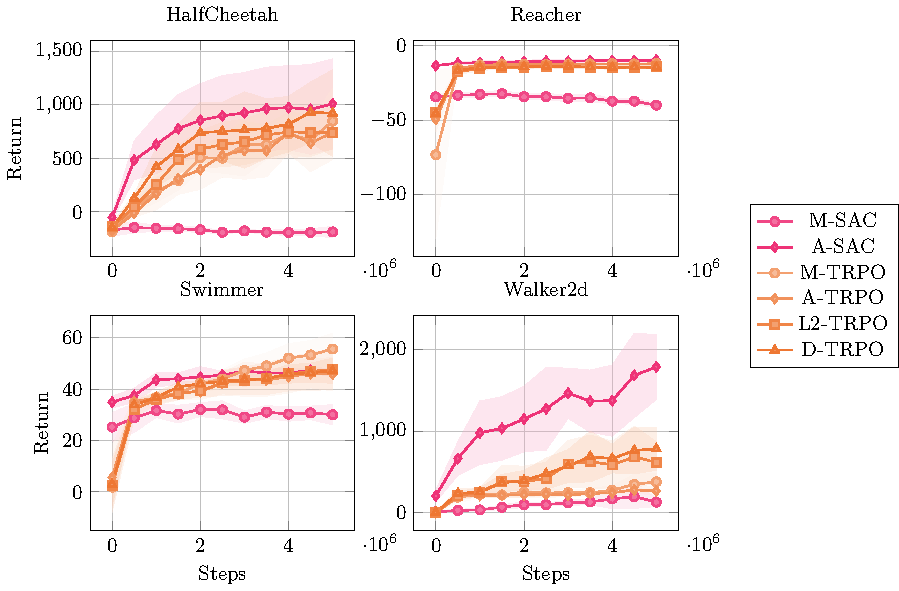
\includegraphics[labelbelief=mdppomdpsets]{img/thesis_plots_belief.pdf}
    \caption{相对于智能体可用信息量的问题维度。
    这些量之间的权衡由黑色虚线表示。
    无延迟\gls{mdp}（$\textbf{U}$）具有完全信息和低维度，而增广状态方法（$\textbf{A}$）是 MDP~\cite{bertsekas1987dynamic,altman1992closed}，具有更高维度。
    无记忆方法（$\textbf{Me}$）维度低，但如\Cref{pp:dmdp_pompd}所示属于\glspl{pomdp}。
    基于模型的方法（$\textbf{Mo}$）同样产生\glspl{pomdp}~\Cref{pp:dmdp_pompd}。
    后一种方法允许在维度和可观测性之间进行权衡。
    }
\label{fig:relations_dmdp_mdp_pomdp}
\end{figure}



\subsection{基于模型方法的反例}
\label{subsec:model_based_sub_optimal}

尽管上一节揭示了负面结果，但人们可能期望 \gls{dmdp} 的特殊结构允许基于模型的方法实现最优性能。
遗憾的是，以下命题证明基于模型策略集合上的最优回报相对于最优基于增广状态策略可能是次优的。

\begin{prop}
\label{pp:counter_example_belief_based}
    设 $\expectedreturn[b][*]$ 为同一 \gls{dmdp} 上基于信念的策略空间的最优回报，$\expectedreturn[a][*]$ 为基于增广状态的策略空间的最优回报。则存在 \glspl{dmdp} 使得
    \begin{align*}
        \expectedreturn[b][*]<\expectedreturn[a][*].
    \end{align*}
\end{prop}
\begin{proof}
    通过给出这样一个 \gls{dmdp} 的实例来证明。
    该实例在\Cref{fig:counter_example_dmdp_pomdp}中展示。
    在该实例中，延迟设为两步。智能体从最下方状态开始，为初始化过程，前两个动作均匀随机选择。在任何状态下，有两个可用动作 $a$ 和 $b$。
    注意，除最上方状态外，没有任何转移产生奖励。
    前者作为吸收态，提供节点上方标注的折扣回报或平均奖励。
    因此，智能体收集的奖励仅取决于其到达的最上方状态。
    除虚线标示的转移外，所有转移都是确定性的。
    在后一种情况下，沿任一路径前进的概率均为 $1/2$。
    该 \gls{mdp} 的特殊之处如下。
    由于两步延迟，初始化后智能体要么处于状态 $s$，要么处于状态 $s'$。
    这意味着，给定 \gls{mdp} 的结构，智能体对其当前状态的信念在 $s$ 和 $s'$ 上各为 $1/2$。
    值得注意的是，基于信念的策略无法区分智能体到达 $s$ 或 $s'$ 所经过的路径。
    第一条路径（红色）从初始状态确定性直接上移到下一个状态，然后转移到 $s$ 或 $s'$。
    第二条路径（蓝色）在第一步向左或向右，然后确定性转移到 $s$ 或 $s'$。
    蓝色路径的有趣特性在于，从第二步起，智能体将知道它会到达 $s$ 还是 $s'$。
    然而，在红色路径上，智能体需要多等待一步才能知道它实际处于 $s$ 还是 $s'$。
    基于信念的智能体无论沿哪条路径都看到相同的状态，而基于增广状态的智能体从增广状态中包含的第一个动作就能知道它将沿蓝色还是红色路径前进。
    因此，基于信念的智能体必须选择一条不考虑路径而优化回报的动作，而基于增广状态的策略可以利用这一额外信息更精细地选择动作。

    智能体需要选择后续两个动作才能获得最终奖励。
    对于红色路径，智能体在选择两个动作时不知道它将沿左分支还是右分支前进。
    智能体在各动作组合下获得的奖励见\Cref{tab:reward_red_path}。
    相反，对于蓝色路径，智能体可以根据其所沿 \gls{mdp} 分支调整第二个动作。
    类似地，\Cref{tab:reward_blue_path}给出了给定第一个动作和观测状态的奖励。
    注意，给定该状态和动作，下一步的最优动作是确定的。

    初始化设计使得智能体沿任一路径的概率相同。
    对于红色路径，智能体应先执行 $b$ 再执行 $a$，获得 $12.5$ 的奖励。
    对于蓝色路径，则应先选择动作 $a$，然后根据观测调整第二个动作，获得 $15$ 的平均奖励，而若先执行 $b$ 则仅获得 $12.5$ 的平均奖励。

    因此，基于增广状态的策略将遵循上述推理，平均获得 $\expectedreturn[a][*]=13.75$ 的奖励。
    基于信念的策略则被迫对两条路径首先选择相同的动作，因为它不知道将沿哪条路径前进。
    若先选择 $a$，智能体在红色路径情况下获得 $10$，在蓝色路径情况下获得 $15$。
    若先选择 $b$，则在红色路径情况下获得 $6.25$，在另一条路径上获得 $12.5$。
    这意味着，无论第一个动作如何选择，期望奖励总是更小。
    其最优回报通过先执行 $a$ 获得，为 $\expectedreturn[b][*]=12.5$。
    证明完毕。
\end{proof}


\begin{figure}[t]
    \centering
    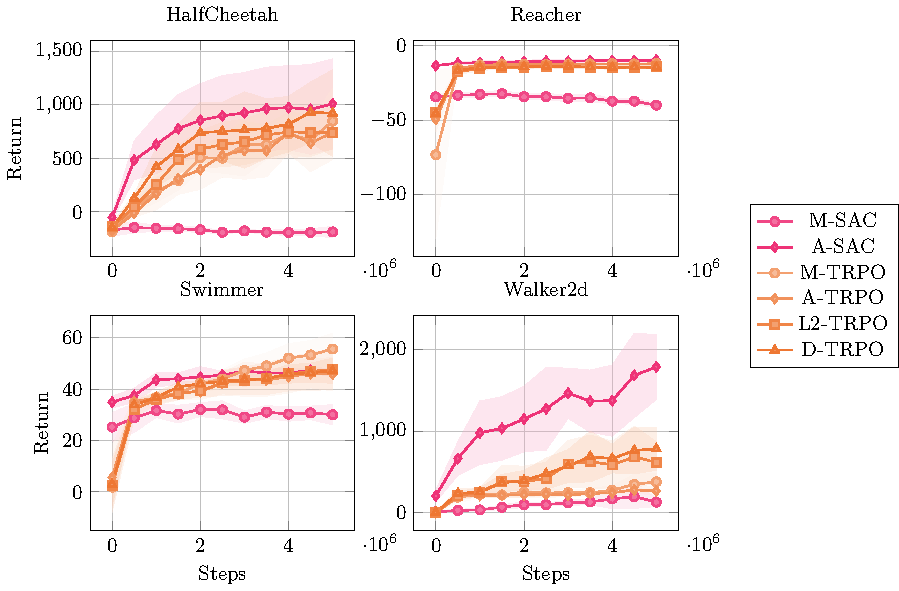
\includegraphics[labelbelief=counterexampledmdppomdp]{img/thesis_plots_belief.pdf}
    \caption{\gls{dmdp}实例，其中对于两步延迟，基于信念的策略相对于最优基于增广状态的策略是次优的。
    在任何状态下，智能体可以选择两个动作 $a$ 和 $b$ 之一。
    除最上方转移外，没有任何转移提供奖励。对于后者，一个循环状态提供节点上方标注的折扣回报或平均奖励。
    除虚线所示转移外，所有转移都是确定性的，其中选择给定动作的智能体各有 $1/2$ 的概率沿任一边前进。
    智能体从最下方状态开始。
    底层\gls{mdp}设计为具有两条路径，它们在状态 $s$ 和 $s'$ 上产生相同的信念。}
    \label{fig:counter_example_dmdp_pomdp}
\end{figure}


\begin{table}[t]
\centering
\begin{tabular}{l|rr}
  & \multicolumn{1}{c}{$a$} & \multicolumn{1}{c}{$b$} \\
\hline
$a$ & $5$ & $10$ \\
$b$ & $12.5$ & $0$ \\
\end{tabular}
\caption{\label{tab:reward_red_path}初始沿红色路径时，所有第一个（行）和第二个（列）动作组合的奖励。}
\end{table}

\begin{table}[t]
\centering
\begin{tabular}{l|rr}
  & \multicolumn{1}{c}{$s$} & \multicolumn{1}{c}{$s'$} \\
\hline
$a$ & $a\rightarrow10$ & $b\rightarrow20$ \\
$b$ & $a\rightarrow15$ & $a\rightarrow10$ \\
\end{tabular}
\caption{\label{tab:reward_blue_path}初始沿蓝色路径时，所有第一个动作（行）与下一步观测状态（列）组合的奖励。第二个动作最优选择并在表中标出。}
\end{table}

尽管这个反例令人沮丧，但本文在\Cref{sec:th_analysis_imitation}中对一种特殊类型的基于信念的策略进行了分析，并证明在光滑性条件下，该策略的回报与最优延迟策略的回报相差不超过一个常数。
